\begin{frame}
  \frametitle{Hybrid $S_N$-Diffusion Method: Theory}
  \textbf{Hybrid $S_N$-Diffusion Method}
  \vspace{.3cm}

  I propose a new hybrid $S_N$-diffusion neutronics method for improving control rod modeling in
  neutron diffusion solvers.

  The hybrid method employs the discrete ordinates ($S_N$) method on subdomains (\textit{correction
  regions}) containing control rods and its vicinity to provide transport corrections to the
  neutron diffusion method.
\end{frame}

\begin{frame}
  \frametitle{Hybrid $S_N$-Diffusion Method: Literature Review}
  \textbf{1-D Discrete Ordinates $\bm{S_N}$ Equation}
  \begin{align}
    \mu_n \frac{d}{dx}&\Psi_g(x, \mu_n) + \Sigma_{t,g}(x)\Psi_g(x, \mu_n) \nonumber \\
                      &=\sum^G_{g'=1} \sum^N_{n'=1} \sum^L_{l=0}
                        \frac{\left(2l+1\right)}{2} \Sigma^{g'\rightarrow g}_{s,l}(x)
                        P_l(\mu_{n'} - \mu_n) w_{n'}\Psi_{g'}(x,\mu_{n'}) \nonumber \\
                      &\qquad + \sum^G_{g'=1} \frac{\chi_g}{2}
                        \frac{\nu\Sigma_{f,g'}(x)}{k} \phi_{g'}(x) + S_g(x,\mu_n)
    \label{eq:1d-sn}
  \end{align}
  \textbf{1-D Neutron Diffusion Equation}
  \begin{align}
    -\frac{d}{dx} D_g(x) \frac{d}{dx} \phi_g(x) + \Sigma_{t,g}(x) \phi_g(x) = \sum^G_{g'=1}&\left[
      \Sigma_s^{g'\rightarrow g}(x)\phi_{g'}(x) + \chi_g\frac{\nu\Sigma_{f,g'}(x)}{k}
    \phi_{g'}(x)\right] \nonumber \\
                                   &+ S_g(x)
    \label{eq:1d-diff}
  \end{align}
\end{frame}

\begin{frame}
  \frametitle{Hybrid $S_N$-Diffusion Method: Theory}
  \textbf{Spatially Varying Diffusion Coefficients}
  \vspace{.3cm}

  Transport corrections are in the form of \textit{Spatially Varying Diffusion Coefficients
  (SVDCs)}, 
  which are identical to the space-dependent diffusion coefficients
  proposed by Ronen:
  %
  \begin{align}
    D^s_g(x) &= -J^{tr}_g(x)\bigg/\frac{d\phi^{tr}_g(x)}{dx}. \label{eq:svdc}
  \end{align}
  %
  where $D^s$ is the \glspl{SVDC}, and the $tr$ superscript denotes neutron
  current and scalar flux computed from the $S_N$ method.
\end{frame}

\begin{frame}
  \frametitle{Hybrid $S_N$-Diffusion Method: Theory}
  \begin{figure}
    \centering
    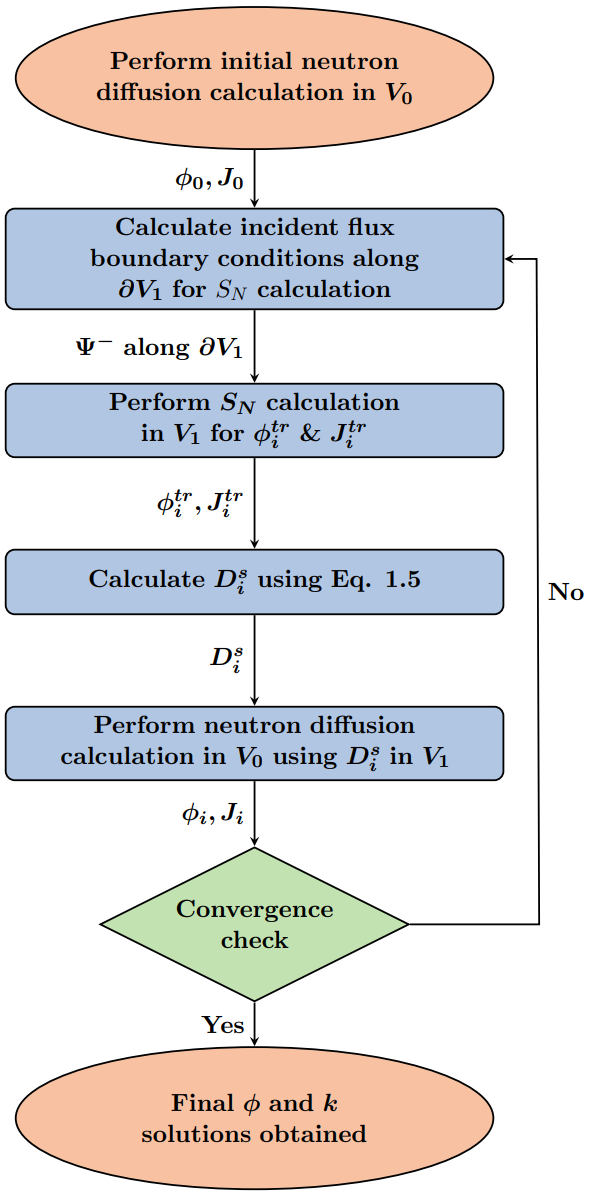
\includegraphics[width=.32\textwidth]{images/algorithm}
    \begin{minipage}[b]{.32\textwidth}
      \caption{Algorithm flowchart for the hybrid $S_N$-diffusion method.}
    \end{minipage}
  \end{figure}
\end{frame}

\begin{frame}
  \frametitle{Hybrid $S_N$-Diffusion Method: Theory}
  \textbf{$S_N$ Subsolver Boundary Conditions}
  \vspace{.3cm}
  \begin{itemize}
    \item In 1-D, the $S_N$ method requires $N/2$ boundary flux parameters per mesh point.
    \item However, the neutron diffusion method can produce at most one independent parameter per
      mesh point.
    %
    \begin{align}
      J_{g,\pm} &= \frac{\phi_g}{4} \mp \frac{D_g}{2}\frac{d\phi_g}{dx} \label{eq:p1-j}
      \shortintertext{where}
      J_{g,\pm} &= \mbox{ neutron forward/backward current of group }g. \nonumber
    \end{align}
    %
  \end{itemize}
  \pause
  $\Rightarrow$ Assume uniformly isotropic transmission of angular flux:
  %
  \begin{align}
    \Psi_g(x,\mu_n) =& J_{g,+}(x)\Bigg/\sum^N_{n=N/2+1}w_n\mu_n && (\mu_n>0) \\
    \Psi_g(x,\mu_n) =& J_{g,-}(x)\Bigg/\sum^{N/2}_{n=1}w_n\mu_n && (\mu_n<0)
  \end{align}
\end{frame}

\begin{frame}
  \frametitle{Hybrid $S_N$-Diffusion Method: Theory}
  \textbf{Correction Region and Buffer Zone}
  \begin{itemize}
    \item Recall that the full problem domain and the correction region are defined as $\Omega^d_0$
      and $\Omega^d_1$, where $\Omega^d_1 \subseteq \Omega^d_0$.
    \item The approximate $S_N$ boundary conditions will generally yield inaccurate flux values
      since realistic reactor systems invariably do not exhibit perfectly isotropic fluxes..
    \item However, the influence of boundary conditions on $J$ and $\frac{d\phi}{dx}$ does not
      extend far from the boundary $\partial\Omega^d_1$ in optically thick media; SVDCs are
      accurate everywhere except near $\partial\Omega^d_1$
  \end{itemize}
  \pause
  $\Rightarrow$ Define $\Omega^d_1$ such that it is large enough to provide sufficient transport
  corrections and accommodate inaccurate SVDCs near $\partial\Omega^d_1$. Discard inaccurate SVDCs
  in favor of the default $P_1$-based diffusion coefficients.
\end{frame}

